\newpage
\sect{8 \quad Random attributes and a direct target ablation}
\textbf{Question and controls.} A new experiment tests variation in the decorations themselves. Every image receives two symbols, placed in legal $5\times5$ boxes with the same one-pixel ink clearance. A bank of 96 templates crosses four geometries (square, diamond, triangle and L), two radii, four angles and three brightness levels. Templates are assigned through balanced shuffles independent of digit labels. Each training image keeps its assigned background. Test digits use the same generation rules with independent seeds, plus two additional redraws at the same sites. These are grayscale intensities.

\begin{center}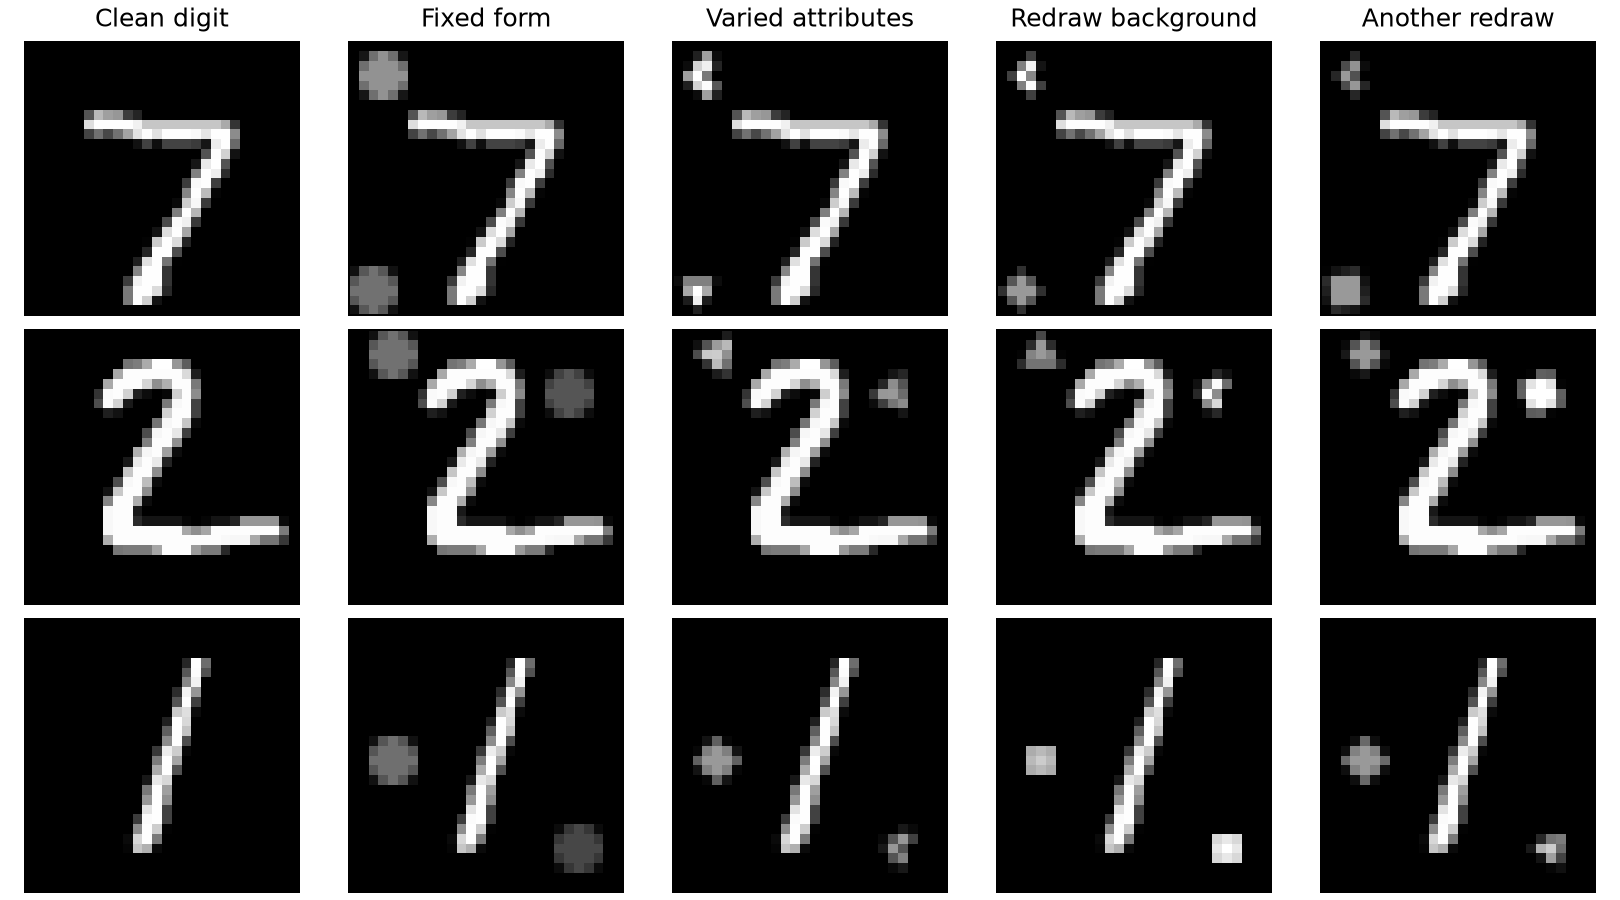
\includegraphics[width=.92\linewidth]{../figures/varied.png}\end{center}
\smallcap{\textbf{Figure 2.} The first three held-out digits. Every stroke and its clearance stay unchanged across columns. Each circular mark in the fixed-form control has the same sum of squared intensities as its corresponding varied symbol. Thus count, location and per-symbol energy match, while occupied area and shape may differ.}

\textbf{Changing the incentive to reconstruct the background.} Hold the marked input fixed and compare reconstruction of the complete image with reconstruction of the original clean digit. The latter is an oracle diagnostic that uses information supplied by the generator [6]. It directly removes the reward for reproducing the added symbols. Cross these targets in pretraining and fine-tuning on varied inputs. Each pair of fine-tuning runs starts from identical weights and cluster centers. Also train ordinary IDEC on clean and fixed-form inputs, the clean-target diagnostic on fixed-form inputs, and the translation and Gaussian interventions on varied inputs.

This gives nine conditions with five seeds each, using the same split, architecture and budgets as Section 5. The \href{https://github.com/JohnR31N/cs126FinalProj/blob/e1cf43f/IDEC/varied/design.md}{protocol was committed before fitting}. We measure accuracy with a frozen training-label map, the fraction of changed cluster assignments across the two redraws, and the decoder's response after each training stage. The response is the reconstruction difference projected onto the actual pixel change, divided by that change's squared norm. One corresponds to fully tracking the changed background. Each image has the same handwriting in every redraw.

\textbf{Limits of the comparison.} The clean target supplies a known clean view and changes both the reconstruction task and its optimization. The attributes are sampled independently of digit labels, while legal site locations depend on the digit silhouette. The experiment covers two small grayscale symbols and one MNIST split. Decoder response measures information used in reconstruction, and leaves other information in the code unmeasured.

\newpage
\sect{9 \quad Random-background results and interpretation}
\begin{center}\small\setlength{\tabcolsep}{4pt}\begin{tabular}{lrrr}
\toprule
Training condition & In-domain ACC & Clean ACC & Redraw flips\\
\midrule
Clean / full target & 73.96 & 73.96 & ---\\
Fixed form / full target & 65.74 & 68.66 & 2.84\\
Varied / full target & 65.40 & 67.47 & 2.98\\
Varied / clean target & 71.44 & 73.14 & 2.35\\
Varied / translation & 77.63 & 78.68 & 1.89\\
Varied / Gaussian & 69.16 & 70.64 & 2.58\\
\bottomrule
\end{tabular}
\end{center}
\smallcap{\textbf{Table 4.} Five-seed means, in percent. In-domain ACC uses the training domain. Clean ACC removes the symbols at test time with the model and mapping fixed. Flips average two redraws of each digit's background.}
Ordinary IDEC fell from 73.96\% on clean digits to 65.74\% with fixed-form backgrounds and 65.40\% with varied backgrounds. The varied-minus-clean difference was $-8.57\pm3.93$ percentage points (paired mean $\pm$ seed SD), negative in every seed. Fixed form was only $0.35\pm4.08$ points above varied geometry, with three seeds favoring it and two favoring varied geometry. The additional effect of geometric diversity at matched energy was inconsistent.

Holding varied inputs fixed, clean reconstruction in both stages raised marked ACC by $6.04\pm4.37$ points to 71.44\% and reduced redraw flips by $0.63\pm0.35$ points to 2.35\%. Every seed agreed on both effects. The decoder's response fell from 0.00828 to 0.00145 in every seed, further suppressing its already weak tracking of the background changes.

\begin{center}\small\setlength{\tabcolsep}{4pt}\begin{tabular}{llrrr}
\toprule
Pretrain target & Fine-tune target & Marked ACC & Redraw flips & Decoder response\\
\midrule
Full & Full & 65.40 & 2.98 & 0.00828\\
Full & Clean & 66.85 & 2.65 & 0.00159\\
Clean & Full & 70.62 & 2.51 & 0.00289\\
Clean & Clean & 71.44 & 2.35 & 0.00145\\
\bottomrule
\end{tabular}
\end{center}
\smallcap{\textbf{Table 5.} Varied-input stage ablation. ACC and flips are percentages. Decoder response measures tracking of a changed background on a scale where one means a full response.}
\textbf{Where the effect enters.} Changing only the fine-tuning target raised ACC by $1.45\pm1.02$ points. Changing only the pretraining target raised it by $5.23\pm4.88$ points. Both increases occurred in every seed. The larger mean effect of changing pretraining suggests that the initialization matters, even when ordinary full-image reconstruction returns during clustering.

\textbf{Augmentation control.} Whole-image translation reached 77.63\% marked ACC and 1.89\% redraw flips, compared with 69.16\% and 2.58\% for Gaussian pretraining. Translation won both comparisons in every seed. Its mean decoder response was 0.00659, above the clean-target arm's 0.00145. Better cluster stability can coexist with a decoder that still responds to decoration.

The target and stage comparisons support a limitation of rewarding these backgrounds during reconstruction. The clean target recovers part of the accuracy gap, while all ten clusters remain occupied.

